\chapter{Selected Realization Aspects}
\label{chap:realization-aspects}

This section describes the design choices of \LibraryName as well as the rationale behind them, and the overarching architecture of the solution. The actual TM implementation is described in detail to make it intuitive. It describes used tools, solutions and algorithms. Additionally, it discusses several interesting problems that were encountered.

\section{System Architecture and Data Workflow}\label{sec:system-architecture}
The project's architecture and data flow are shown in Figure \ref{fig:projectdiagram}. The design is split between a \textbf{host (PC)} and an \textbf{embedded device}, allowing models to be developed on one platform and transferred to different hardware for deployment.

\paragraph{Training and exporting}
The process starts by defining and training TM models using an external library (\textbf{C}). In this project, we use the \GreenTsetlinName library. Once training is complete, our Python Interface (\textbf{G}) handles exporting the model. We support two different interchange formats:
\begin{compactitem}
    \item FlatBuffers~\cite{flatbuffers} (\textbf{D}) - An efficient, cross-platform serialization format utilizing a third-party library.
    \item Custom Binary (\textbf{E}) - A dependency-free format that may require adjustments based on the target hardware.
\end{compactitem}

\paragraph{On-device execution}
After the serialized model state (\textbf{I}) is saved, it can be moved to the embedded device. On the device, we use our core library (\textbf{O}), which supports every step of the machine learning workflow:
\begin{compactitem}
    \item It can load a pretrained model (\textbf{K}) to start making predictions (\textbf{N}) immediately.
    \item It can be trained further on the device (\textbf{L}) using data gathered during operation (\textbf{P}).
    \item It can save and export the updated model state (\textbf{M}) to back up or inspect what the device has learned.
    \item It also supports creating new models (\textbf{J}) directly on the device if needed.
\end{compactitem}

\paragraph{Python integration}
Since the core library is self-sufficient, it can also be compiled for the host architecture. This allows us to provide a Python package with bindings to the same C code, so that it can run on a standard computer. This package includes a \textit{Scikit-learn}-like interface (\textbf{F}) and is easy to install, similar to other common machine learning tools. This enables rapid testing of ideas in \textit{Jupyter Notebooks} (\textbf{H}) and makes it possible to benchmark our implementation against standard models provided by Python libraries.

\begin{figure}[!htbp]
\centering
\begin{tikzpicture}[scale=0.7, transform shape]
\pgfdeclarelayer{background}
\pgfsetlayers{background,main}
\tikzset{refnode/.style={circle, draw, fill=white, inner sep=1pt, font=\scriptsize\bfseries}}

\node [
    draw,
    rectangle,
    align=center,
] (tsetlinmachine) {TM\\Model Definition};
\node [refnode] at (tsetlinmachine.north east) {A};

\node [
    draw,
    rectangle,
    align=center,
    below=0.5cm of tsetlinmachine,
] (trainer) {Training Process};
\node [refnode] at (trainer.north east) {B};

\node [
    draw,
    dotted,
    rectangle,
    align=center,
    below=1cm of trainer,
] (traindata) {Training\\Data};

\node [
    draw,
    dotted,
    rectangle,
    align=center,
    left=0.75cm of traindata,
] (evaldata) {Evaluation\\Data};

\begin{pgfonlayer}{background}
\node [
    draw,
    dashed,
    rectangle,
    inner sep=0.5cm,
    fit=(tsetlinmachine) (trainer),
    label=above:External Library,
    fill=green!10,
] (greentsetlin) {};
\end{pgfonlayer}
\node [refnode] at (greentsetlin.north east) {C};

\node [
    draw,
    rectangle,
    align=center,
    right=1.75cm of tsetlinmachine,
    yshift=-0.25cm,
] (savetofbs) {Export Model\\as FlatBuffers};
\node [refnode] at (savetofbs.north east) {D};

\node [
    draw,
    rectangle,
    align=center,
    below=1.25cm of savetofbs,
] (savetobin) {Export Model\\as Binary};
\node [refnode] at (savetobin.north east) {E};

\node [
    draw,
    rectangle,
    align=center,
    right=5.5cm of trainer,
] (ctsetlinclassifier) {Scikit-learn\\Interface for\\the C Core};
\node [refnode] at (ctsetlinclassifier.north east) {F};

\begin{pgfonlayer}{background}
\node [
    draw,
    dashed,
    rectangle,
    inner sep=0.5cm,
    label=above:Python Interface,
    fit=(savetofbs) (savetobin) (ctsetlinclassifier),
    fill=blue!10,
] (tsetlinmachinepy) {};
\end{pgfonlayer}
\node [refnode] at (tsetlinmachinepy.north east) {G};

\node [
    draw,
    rectangle,
    align=center,
    above=2.5cm of ctsetlinclassifier,
] (jupyternotebook) {Jupyter Notebook\\Integration};
\node [refnode] at (jupyternotebook.north east) {H};

\node [
    draw,
    dotted,
    rectangle,
    align=center,
    below=6cm of savetobin,
    xshift=2cm,
] (modelstate) {Serialized\\Model State};
\node [refnode] at (modelstate.north east) {I};

\node [
    draw,
    dashed,
    rectangle,
    fit=(greentsetlin) (tsetlinmachinepy) (traindata) (evaldata) (jupyternotebook),
    inner sep=0.75cm,
    label=above:\textbf{Host (PC)},
] (host) {};

\node [
    draw,
    rectangle,
    align=center,
    left=2.5cm of modelstate,
] (tmload) {Load\\Model State};
\node [refnode] at (tmload.north east) {K};

\node [
    draw,
    rectangle,
    align=center,
    above=0.5cm of tmload,
] (tmcreate) {TM\\Model Definition};
\node [refnode] at (tmcreate.north east) {J};

\node [
    draw,
    rectangle,
    align=center,
    below=0.5cm of tmload,
] (tmtrain) {On-Device\\Training};
\node [refnode] at (tmtrain.north east) {L};

\node [
    draw,
    dotted,
    rectangle,
    align=center,
    left=1.75cm of tmtrain,
] (externaldata) {External\\Data};
\node [refnode] at (externaldata.north east) {P};

\node [
    draw,
    rectangle,
    align=center,
    below=0.5cm of tmtrain,
] (tmsave) {Save\\Model State};
\node [refnode] at (tmsave.north east) {M};

\node [
    draw,
    rectangle,
    align=center,
    below=0.5cm of tmsave,
] (tmpredict) {TM\\Model Inference};
\node [refnode] at (tmpredict.north east) {N};

\node [
    draw,
    dotted,
    rectangle,
    align=center,
    left=1.25cm of tmpredict,
] (modeloutput) {Prediction\\Results};
\node [refnode] at (modeloutput.north east) {R};

\begin{pgfonlayer}{background}
\node [
    draw,
    dashed,
    rectangle,
    inner sep=0.5cm,
    label=above:Core Library in C,
    fit=(tmload) (tmtrain) (tmsave) (tmpredict) (tmcreate),
    fill=yellow!10,
] (tsetlinmachinec) {};
\end{pgfonlayer}
\node [refnode] at (tsetlinmachinec.north east) {O};

\node [
    draw,
    dashed,
    rectangle,
    fit=(tsetlinmachinec) (externaldata),
    inner sep=0.75cm,
    label=above:\textbf{Embedded (On-Device)},
] (embedded) {};

\begin{scope}[->, very thick]
\draw [->] (tsetlinmachine.south) -| (trainer.north);

\draw [->] (traindata.north) -| (trainer.south);
\draw [->] (evaldata.north) |- (trainer.west);

\draw [->] (trainer.east) -| (savetofbs.south);
\draw [->] (trainer.east) -| (savetobin.north);

\draw [->] (savetofbs.east) -| (modelstate.north);
\draw [->] (savetobin.east) -| (modelstate.north);

\draw [->] (ctsetlinclassifier.north) -| (jupyternotebook.south);
\draw [->, dotted] (tsetlinmachinec.south east) -| (ctsetlinclassifier.south) node[near start, above] {Python Bindings};

\draw [->] (modelstate.west) |- (tmload.east);
\draw [->] (tmsave.east) -| (modelstate.south);

\draw [->] (tmload.south) -| (tmtrain.north);
\draw [->] (tmload.south) -| (tmtrain.north);
\draw [->] (tmtrain.south) -| (tmsave.north);

\draw [->] (externaldata.east) |- (tmtrain.west);
\draw [->] (tmpredict.west) |- (modeloutput.east);
\end{scope}

\end{tikzpicture}

\caption[System architecture and data workflow]{System architecture and data workflow. Models can be pretrained using \GreenTsetlinName library (C). We provide a Python Interface (G) that handles model serialization and includes a Scikit-learn compatible wrapper. Our Core TM Library (O), implemented in the C programming language, executes the model on the target device, supporting both inference and on-device training.}
\label{fig:projectdiagram}
\end{figure}
\FloatBarrier

\section{Design}\label{sec:design}
Even though optimization was the primary objective, not every method could be utilized due to the target environments having very limited resources and hardware limitations. In particular, vectorization was completely out of the picture, even though \GreenTsetlinName has it enabled by default. GPU programming was obviously dismissed for the same reason -- although notably, such an implementation is possible~\cite{granmo2020pytsetlinmachinecuda}.

\subsection{Programming Language}
Since the thesis topic requires \LibraryName to be designed for embedded devices, there were only a few suitable options like C/C++, Rust or MicroPython. C was chosen as the most widely used language for embedded systems -- it is efficient, lightweight and portable. Its popularity also means it has extensive third party library support. The authors' previous experience working with C/C++ also influenced this decision.  
Exporting models from \GreenTsetlinName is done in Python, as it is a Python library.  
\LibraryName also has Python bindings so that it can be used conveniently from Python.

\subsection{Execution Engine}
Even though there exists a number of existing libraries implementing the Tsetlin Machines, \LibraryName was essentially created from the ground up without taking much inspiration or hints from them. It was required to be written primarily with optimization in mind so that it works as fast as possible while maintaining small size and portability on top of utilizing little power and memory.

It was also decided \LibraryName should support multiple different TM variants so their efficiency could be tested -- Coalesced, Sparse and Stateless.

\subsection{Model Serialization Library}
Several libraries were compiled and compared as possible options to implement the model serialization format. Only C libraries were taken into consideration. See Table~\ref{tab:serial-lib-comp}.

\begin{table}[!htbp]
\centering
\caption[Comparison of model serialization libraries]{Comparison of selected model serialization libraries\label{tab:serial-lib-comp}}
\begin{tabularx}{\textwidth}{@{}L L L L L@{}} \toprule
    \textbf{Format name} & \textbf{Comment} & \textbf{Schema complexity} & \textbf{Efficiency on edge device} & \textbf{Library size on edge device} \\ \midrule \midrule
    Protocol Buffers & Simple and small model representation & Low & Fast but needs object parsing & Too big \\ \midrule
    ONNX & A standardized way to store models and operation graphs & High & Low - needs graph and tensor parsing & Much too big \\ \midrule
    FlatBuffers & ``Protocol buffers lite'' & Low & Very fast, zero-copy & Acceptable \\ \bottomrule
\end{tabularx}
\end{table}

\section{TM implementation}
This section describes the implementation of the different TM types. Each type is broken down into its main components, and provides technical intuition about their operation.

\subsection{Tsetlin Automaton}
A Tsetlin Automaton is the smallest part of a TM, and it is what clauses consist of. Implementation-wise it is represented by a singular, 8-bit integer, meaning its values can range from -127 to 127 by default. The range can be made smaller by setting model parameters $max\_state$ and $min\_state$. 
Further on in this thesis, the term that a Tsetlin Automaton is active, means its internal integer value is greater or equal than halfway between $max\_state$ and $min\_state$; $value \ge \frac{max\_state + min\_state}{2}$. 
One input bit on position $i$ has two corresponding Tsetlin Automata at positions in clause $2 \times i$ and $2 \times i + 1$. The first one -- positive -- decides whether the input bit -- $x_i$ -- should be included in the clause, and the other -- negative -- whether its negation -- $\neg x_i$ -- should be included.

\subsection{Coalesced TM}
Coalesced TM is the variant most closely resembling the original TM out of those implemented by \LibraryName. The implementation closely follows the paper~\cite{glimsdal2021coalescedmultioutputtsetlinmachines}.

\subsubsection{Training}
The training loop consists of three distinct steps repeated for each datapoint, further explained below.
\begin{compactenum}
    \item Calculate clause output.
    \item Sum votes.
    \item Calculate and apply feedback.
\end{compactenum}

\paragraph{Calculate Clause Output}
The current states of Tsetlin Automata in each clause are used to determine whether the clause activates -- 1, or not -- 0. This output is temporarily stored in an internal array. 
For this step specifically, a clause is active if either of two conditions is met:
\begin{compactitem}
    \item \textbf{The clause is empty} -- no Tsetlin Automaton is active.
    \item For the training input datapoint, all bits corresponding to active positive Tsetlin Automata of this clause are set and all bits corresponding to active negative Tsetlin Automata of this clause are unset.
\end{compactitem}

\paragraph{Sum Votes}
This step uses the information calculated in the previous point whether clauses are active or not. Active clauses vote for all possible classes with trained weights. Specifically, clause $i$ votes for class $j$ with trained weight $w_{i,j}$. $w_{i,j}$ can be positive or negative. 
As all active clauses vote, each class accumulates their votes. The sum of votes is then clipped to parameter $threshold$. It serves the same purpose as gradient clipping in other ML architectures, mainly for numerical stability. %TODO: citation

\paragraph{Calculate and Apply Feedback}
As the sum of votes indicates whether a class should be chosen or not, that prediction can be compared to the actual datapoint label. Based on this information, a suitable feedback to be applied to Tsetlin Automata. 
For each datapoint two classes are specified for feedback:
\begin{compactitem}
    \item Positive -- one of the classes, or the one class, specified by label.
    \item Negative -- one of the classes not specified by label.
\end{compactitem}
Both have a chance to trigger feedback to all clauses. 
For the positive class, the chance is inversely proportional to the clipped sum of votes it received. That means the model applies feedback more often the \textit{less} sure it is the class is correct. Although unintuitive at first, this practice is used to avoid overfitting. 
For the negative class, the chance is proportional to the clipped sum of votes it received. This means the model applies feedback more often the more sure it is the class is incorrect.

What is unique to \LibraryName, it allows both predictions and output to be customized to be any type of data. 
A custom feedback function can be set for the model, to override how positive and negative classes are chosen. The default uses normal classification, where the output and prediction is an integer identifying a class. 
Another predefined function allows multi-class classification, where output and prediction is an 8-bit integer array where the length is the number of classes, where value 1 signifies a class with a given identifier being chosen, value 0 -- not chosen. 
Also a custom comparison function can be set for the model, to override when the output and prediction data classes should be treated as equal. By default a simple memory comparison is used, which handles the vast majority of uses -- even when fully customized.

\paragraph{Feedback}\label{feedback-dense}
When a chosen class triggers feedback to all clauses, for each clause separately one of three feedback types may be applied. 
Tsetlin Automata changes specified in \textbf{Action} are not always changed -- they have a random chance to do so based on the parameter \textit{s} -- sensitivity -- further explained in \textbf{Sensitivity} for each feedback type.
\begin{compactitem}
\item \textbf{Type Ia}
    \begin{compactitem}
        \item \textbf{Condition:} The clause is active and voted correctly for the chosen class (with the correct weight sign).
        \item \textbf{Action:} Reinforce Tsetlin Automata making up the clause, reinforce weight for the chosen class.
        \item \textbf{Sensitivity:} The chance for change is either $\frac{1}{s}$ for true positive and true negative Tsetlin Automata, and otherwise its inversion -- $\frac{s - 1}{s}$. Model parameter \textit{boost\-\_true\-\_positive} makes it so that true positive Tsetlin Automata are always changed.
        \item \textbf{Intuition:} The clause should continue to vote for the same class.
    \end{compactitem}
\item \textbf{Type Ib}
    \begin{compactitem}
        \item \textbf{Condition:} The clause is inactive and (would have) voted correctly for the chosen class.
        \item \textbf{Action:} Lower the confidence of all the Tsetlin Automata making up the clause, positive and negative.
        \item \textbf{Sensitivity:} The chance for change is always $\frac{1}{s}$.
        \item \textbf{Intuition:} The clause should ``find something else to do'', countering force.
    \end{compactitem}
\item \textbf{Type II}
    \begin{compactitem}
        \item \textbf{Condition:} The clause is active and voted incorrectly for the chosen class.
        \item \textbf{Action:} Raise, towards activation, inactive Tsetlin Automatons that could deactivate the clause for this datapoint, punish the weight of the chosen class towards zero.
        \item \textbf{Sensitivity:} Change always happens.
        \item \textbf{Intuition:} Try two things at once: exclude the clause and fix the weight (flip the sign). Although these goals are opposing, just one of them needs to come true, and the hope is one of them should do so before the other.
    \end{compactitem}
\item Nothing happens if the clause is inactive and would have voted incorrectly.
\end{compactitem}

\subsubsection{Inference}
Inference on a datapoint looks very similar to training, with few key differences.
\begin{compactenum}
    \item Calculate clause output
    \item Sum votes
    \item Apply output activation
\end{compactenum}

\paragraph{Calculate Clause Output}
Unlike in training, an empty clause -- with no active Tsetlin Automata -- is inactive. Otherwise it does the same thing -- calculates which clauses are active with a given input.

\paragraph{Sum Votes}
Exactly the same as training. Sums up class votes from active clauses.

\paragraph{Apply Output Activation}
Applies a function to determine the output from the summed up class votes. By default, it simply returns an integer -- an identifier of a class with the most votes.

Again, this can be fully customized. A custom output activation function can be set for the model, to override what the model outputs based on the summed up weights.

Another predefined function allows multi-class classification, where the output is an 8-bit integer array where the length is the number of classes, where value 1 signifies a class with a given identifier being chosen, value 0 - not chosen.

\subsubsection{Data Layout}
A clause is represented as a simple array of Tsetlin Automata states. For the sake of efficiency they are ordered by the literals they correspond to, in pairs of positive and negative Tsetlin Automata. This simplified representation is visualized in Figure~\ref{fig:dense-data-layout}.

The \textit{i}-th array field represents the state of Tsetlin Automaton corresponding to literal with index $\lfloor \frac{i}{2} \rfloor$ -- positive if \textit{i} is even, negative if odd.

\begin{figure}[!htbp]
\centering
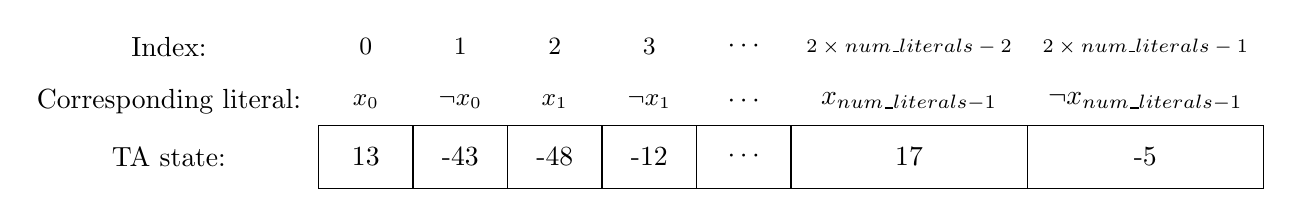
\begin{tikzpicture}
    % Indices
    \foreach \i in {0,1,2,3} {
        \node at (\i*1.2,0.7) {\small \i};
    }
    \node at (4*1.2,0.7) {$\cdots$};
    \node at (6.9,0.7) {\scriptsize $2 \times num\_literals - 2$};
    \node at (9.9,0.7) {\scriptsize $2 \times num\_literals - 1$};
    
    % Literals
    \node at (0*1.2,0) {\small $x_0$};
    \node at (1*1.2,0) {\small $\neg x_0$};
    \node at (2*1.2,0) {\small $x_1$};
    \node at (3*1.2,0) {\small $\neg x_1$};
    \node at (4*1.2,0) {$\cdots$};
    \node at (6.9,0) { $x_{num\_literals - 1}$};
    \node at (9.9,0) { $\neg x_{num\_literals - 1}$};
    
    % States
    \foreach \i/\v in {
            0/13,1/-43,
            2/-48,3/-12,
            4/$\cdots$
            } {
        \node[draw, minimum width=1.2cm, minimum height=0.8cm] (cell\i) at (\i*1.2,-0.7) {\v};
    }
    \node[draw, minimum width=3cm, minimum height=0.8cm] (cell5) at (6.9,-0.7) {17};
    \node[draw, minimum width=3cm, minimum height=0.8cm] (cell6) at (9.9,-0.7) {-5};

    % Labels
    \node at (-2.5,0.7) {Index:};
    \node at (-2.5,0) {Corresponding literal:};
    \node at (-2.5,-0.7) {TA state:};
\end{tikzpicture}
\caption{Clause data layout of Coalesced TM}
\label{fig:dense-data-layout}
\end{figure}

\subsubsection{Model Serialization Format}

The model state is represented by the FlatBuffers schema in Listing~\ref{lst:dense-schema}. It defines the model parameters, clause weights, and the internal states of the Tsetlin Automata.

\begin{listing}[!htbp]
    \caption[Coalesced TM FlatBuffers serialization format]{Coalesced TM FlatBuffers serialization format\label{lst:dense-schema}}
    \begin{minted}[escapeinside=||, fontfamily=tt]{text}
|\kw{table}| Parameters {
  threshold:  |\tp{uint}|;  |\cm{// tsetlin automaton threshold}|
  n_literals: |\tp{uint}|;  |\cm{// total number of literals}|
  n_clauses:  |\tp{uint}|;  |\cm{// total number of clauses}|
  n_classes:  |\tp{uint}|;  |\cm{// number of output classes}|
  max_state:  |\tp{byte}|;  |\cm{// maximum state for automaton}|
  min_state:  |\tp{byte}|;  |\cm{// minimum state for automaton}|
  boost_tp:   |\tp{ubyte}|; |\cm{// boost true positive feedback}|
  learn_s:    |\tp{float}|; |\cm{// learning sensitivity (s)}|
}
|\kw{table}| ClauseWeightsTensor {
  weights: [|\tp{short}|]; |\cm{// clause weights}|
  shape:   [|\tp{uint}|];  |\cm{// dimensions e.g. [n\_clauses, n\_classes]}|
}
|\kw{table}| AutomatonStatesTensor {
  states: [|\tp{byte}|]; |\cm{// automaton states}|
  shape:  [|\tp{uint}|]; |\cm{// dimensions e.g. [n\_clauses, n\_literals, 2]}|
}
|\kw{table}| Model {
  params:           Parameters            (|\tp{required}|); |\cm{// model parameters}|
  automaton_states: AutomatonStatesTensor (|\tp{required}|); |\cm{// automaton states}|
  clause_weights:   ClauseWeightsTensor   (|\tp{required}|); |\cm{// clause weights}|
  literal_names:    [|\tp{string}|];                         |\cm{// names of literals}|
}
|\kw{root\_type}| Model;
    \end{minted}
\end{listing}

\subsection{Sparse TM}
A Sparse TM~\cite{glimsdal2024sparsetsetlinmachine} aims to efficiently process sparse data. It uses the same core principles and mechanics as the Coalesced TM, its main difference being the underlying data layout. It also introduces \textit{Active Literals} -- it functions as a list of literals considered to be added to sparse state. Notably, both sparse state and \textit{Active Literals} need to have a limited size or the model is slower and larger than Coalesced TM, and learns poorly -- something not mentioned in the paper~\cite{glimsdal2024sparsetsetlinmachine}.

\subsubsection{Data Layout}
Unlike the Coalesced TM, the Sparse TM does not store all Tsetlin Automata. Simply put, it only keeps the Tsetlin Automata, which state is above a certain threshold. By doing so, in principle it does not need to waste space and computation power for Tsetlin Automata it deems unlikely to become active for a given clause. The simplified structure is shown in figure ~\ref{fig:sparse-data-layout}

Since not all Tsetlin Automata are present in a clause a linked list is used as the underlying data structure. Identifying indices cannot be inferred from the data structure and need to be stored in nodes.

\begin{figure}[!htbp]
\centering
\begin{tikzpicture}
    
    % Literals
    \node at (0*1.8,0) { $\neg x_{0}$};
    \node at (1*1.8,0) { $x_{2}$};
    \node at (2*1.8,0) { $\neg x_{11}$};
    \node at (3*1.8,0) { $\neg x_{21}$};
    \node at (4*1.8,0) { $\cdots$};
    \node at (5*1.8,0) { $x_{28}$};
    
    % Indices
    \foreach \i/\v in {
            0/1,1/4,
            2/23,3/43,
            4/$\cdots$,
            5/56
            } {
        \node[draw, minimum width=1.0cm, minimum height=0.6cm] (id\i) at (\i*1.8,-0.7) {\v};
    }
    
    % States
    \foreach \i/\v in {
            0/13,1/-43,
            2/-48,3/-12,
            4/$\cdots$,
            5/-48
            } {
        \node[draw, minimum width=1.0cm, minimum height=0.6cm] (state\i) at (\i*1.8,-1.4) {\v};
    }
    
    % Pointer
    \foreach \i/\v in {
            0/\textit{next},1/\textit{next},
            2/\textit{next},3/\textit{next},
            4/$\cdots$,
            5/\textit{null}
            } {
        \node[draw, minimum width=1.0cm, minimum height=0.6cm] (ptr\i) at (\i*1.8,-2.1) {\v};
    }

    \foreach \i in {0,1,2,3,4,5} {
        \node[draw, fit=(id\i) (state\i) (ptr\i)] (cell\i) {};
    }

    \draw [->] (ptr0.east)  -| ++(.4, .7) -- (cell1.west);
    \draw [->] (ptr1.east)  -| ++(.4, .7) -- (cell2.west);
    \draw [->] (ptr2.east)  -| ++(.4, .7) -- (cell3.west);
    \draw [->, dashed] (ptr3.east)  -| ++(.4, .7) -- (cell4.west);
    \draw [->, dashed] (ptr4.east)  -| ++(.4, .7) -- (cell5.west);

    % Labels
    \node at (-2.5,0) {Corresponding literal:};
    \node at (-2.5,-0.7) {Index:};
    \node at (-2.5,-1.4) {TA state:};
    \node at (-2.5,-2.1) {Pointer:};
\end{tikzpicture}
\caption{Clause data layout of Sparse TM}
\label{fig:sparse-data-layout}
\end{figure}

\subsubsection{Training}
Aside from obvious changes from Coalesced TM needed to accommodate the different data structure, the feedback mechanism has some modifications. Namely, a new Tsetlin Automaton can be introduced to a clause only in type Ia of feedback, only when the corresponding literal currently belongs to Active Literals of a class which triggered this feedback. A literal can be added to \textit{Active Literals} in feedback type II. \textit{Active Literals} are not being explicitly removed, but the oldest is replaced when adding a new one.

\subsection{Stateless TM}
A Stateless TM is a slimmed down version of Sparse TM that does not allow any model training, at the same time further reducing model size to the smallest and fastest possible for inference. It should only be created from a trained model of a different TM variant.

\subsubsection{Data Layout}
Stateless TM, as the name suggests, does not store Tsetlin Automaton states at all. Here a degenerated version of Tsetlin Automaton is active if it is present at all. The simplified structure is shown in figure ~\ref{fig:stateless-data-layout}

\begin{figure}[!htbp]
\centering
\begin{tikzpicture}
    % Literals
    \node at (0*1.8,0) { $\neg x_{0}$};
    \node at (1*1.8,0) { $x_{2}$};
    \node at (2*1.8,0) { $\neg x_{11}$};
    \node at (3*1.8,0) { $\neg x_{21}$};
    \node at (4*1.8,0) { $\cdots$};
    \node at (5*1.8,0) { $x_{28}$};
    
    % Indices
    \foreach \i/\v in {
            0/1,1/4,
            2/23,3/43,
            4/$\cdots$,
            5/56
            } {
        \node[draw, minimum width=1.0cm, minimum height=0.6cm] (id\i) at (\i*1.8,-0.7) {\v};
    }
    
    % Pointer
    \foreach \i/\v in {
            0/\textit{next},1/\textit{next},
            2/\textit{next},3/\textit{next},
            4/$\cdots$,
            5/\textit{null}
            } {
        \node[draw, minimum width=1.0cm, minimum height=0.6cm] (ptr\i) at (\i*1.8,-1.4) {\v};
    }

    % Fit node with increased inner sep for padding
    \foreach \i in {0,1,2,3,4,5} {
        % inner sep=3pt adds the gap you're looking for
        \node[draw, fit=(id\i) (ptr\i), inner sep=3pt, rounded corners=1pt] (cell\i) {};
    }

    % Arrows: Adjusted path to account for the extra padding
    \draw [->] (ptr0.east)  -| ++(.45, .35) -- (cell1.west);
    \draw [->] (ptr1.east)  -| ++(.45, .35) -- (cell2.west);
    \draw [->] (ptr2.east)  -| ++(.45, .35) -- (cell3.west);
    \draw [->, dashed] (ptr3.east)  -| ++(.45, .35) -- (cell4.west);
    \draw [->, dashed] (ptr4.east)  -| ++(.45, .35) -- (cell5.west);

    % Labels
    \node[anchor=east] at (-1.2, 0) {Corresponding literal:};
    \node[anchor=east] at (-1.2, -0.7) {Index:};
    \node[anchor=east] at (-1.2, -1.4) {Pointer:};
\end{tikzpicture}
\caption{Clause data layout of Sparse TM (Stateless)}
\label{fig:stateless-data-layout}
\end{figure}

\section{Optimizations}
Seeing as speed, size, portability as well as limiting the usage of power and memory were all key requirements, optimizations were the main focus of this project. In this section a few of the more interesting examples are listed.

\subsection{Pseudo Random Number Generation}
Analyzing the efficiency of a development version with valgrind and callgrind, it was obvious that most training time was spent on calls to \textit{rand()} - pseudo random number generation. 
While it is not costly to call once, the cost quickly accumulates over millions of calls.

\subsubsection{Analysis}
\textit{rand()} is costly because it aims for a uniform spread, as evenly as possible. \LibraryName intentionally adopts a design that relaxes this uniformity, accepting minor statistical deviations that average out over millions of calls -- in order to prioritize execution speed and reduced power consumption. The pseudo random number generation for this purpose does not need to be cryptographically secure either -- \textit{rand()} is not anyway. 
A quick look at \GreenTsetlinName revealed that it suffered from the same problem. Its solution was to use a \texttt{wyhash64} algorithm. Using just an 64-bit integer addition, two 128-bit integer multiplications and few bitwise operations as well as a double multiplication, it is overall a much cheaper solution. 
Listing ~\ref{lst:wyhash64} shows the \GreenTsetlinName implementation of \texttt{wyhash64}.
\begin{listing}[!htbp]
    \caption[\GreenTsetlinName implementation of \texttt{wyhash64}]{\GreenTsetlinName implementation of \texttt{wyhash64}\label{lst:wyhash64}}
    \begin{minted}{c}
double next_u()
{
    wyhash64_x += 0x60bee2bee120fc15;
    __uint128_t tmp;
    tmp = (__uint128_t) wyhash64_x * 0xa3b195354a39b70d;
    uint64_t m1 = (tmp >> 64) ^ tmp;
    tmp = (__uint128_t)m1 * 0x1b03738712fad5c9;
    uint64_t m2 = ((tmp >> 64) ^ tmp);

    double r = 0x1.0p-64 * m2;
    return r;
}
    \end{minted}
\end{listing}

\subsubsection{Solution}
\texttt{Wyhash64} represents a significantly lower-cost solution compared to the alternative; however, its computational and energy costs remain non-negligible. 128-bit integer multiplications and double multiplication cost many precious CPU cycles which means time and power. 
Listing ~\ref{lst:fast-prng} shows the \LibraryName implementation of \texttt{xorshift32}. 
All that is really needed are a few bit shifts and XOR operations. It uses so few CPU cycles it is basically free. It might also be the case one of the authors likes low-level optimization an unhealthy amount. 

\begin{listing}[!htbp]
    \caption[\LibraryName implementation of \texttt{xorshift32}]{\LibraryName implementation of \texttt{xorshift32}\label{lst:fast-prng}}
    \begin{minted}{c}
uint32_t prng_next_uint32(struct FastPRNG* prng) {
    uint32_t x = prng->state;
    x ^= x << 13;
    x ^= x >> 17;
    x ^= x << 5;
    prng->state = x;
    return x;
}

float prng_next_float(struct FastPRNG* prng) {
    uint32_t x = prng->state;
    x ^= x << 13;
    x ^= x >> 17;
    x ^= x << 5;
    prng->state = x;
    static union {
        uint32_t u32;
        float f;
    } caster;
    /* Reinterpret x as float: keep random mantissa, set exponent to 127
       (1.0f), then subtract 1.0f to obtain value in [0,1).
    */
    caster.u32 = 0x3F800000 | x >> 9;

    return caster.f - 1.0f;
}
    \end{minted}
\end{listing}


\section{Summary}
In conclusion, \LibraryName is a C library designed for resource-limited systems, using FlatBuffers format for model serialization. It can be used conveniently from Python on the host device, both inference and training is available from C on the edge device, and models can be transferred between them -- as shown in Section~\ref{sec:system-architecture}. 
This chapter furthermore touches on the actual, low-level implementation of TM types. Notable optimizations are also explained here.